\chapter{Problema 2}

\section{Little Bishops}

Un alfil es una pieza utilizada en el juego de ajedrez el cual es jugado en una tabla con grillas cuadradas. Un alfil puede moverse solamente de forma diagonal desde su posici�n actual, y dos alfiles se atacan si uno de ellos est� en el camino del otro. En la siguiente figura, los cuadrados negros representan los lugares alcanzables por el alfil $B_1$ desde su posici�n actual. La figura tambi�n muestra que los alfiles $B_1$ y $B_2$ est�n en posiciones de ataque, pero $B_1$ y $B_3$ no. $B_2$ y $B_3$ tampoco se atacan.

\begin{figure}[H]
\centering
\label{ej2_tableroEnunciado}
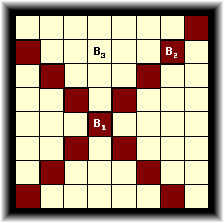
\includegraphics[scale=0.5]{./graficos/ej2/tableroEnunciado.jpg}
\end{figure}

Ahora, dados dos n�meros \textbf{n} y \textbf{k}, su deber es determinar la cantidad de formas en que uno puede ubicar $k$ alfiles en un tablero de ajedrez de $n � n$, de forma tal que ningun par de ellos se atacan.
 
\textbf{Entrada:}

El archivo de entrada puede contener m�ltiples casos de test. Cada test ocupa una l�nea en el archivo de entrada y contiene dos enteros \textbf{n} $(1 \le n \le 8)$ y \textbf{k} $(0 \le k \le n^2)$. 

Un caso de test que contiene dos ceros para n y k finaliza la entrada y no necesitar� procesar esta particular entrada.
 
\textbf{Salida:}

Para cada caso de test en la entrada imprimir una l�nea conteniendo el n�mero total de formas en la cual uno puede ubicar la cantidad de alfiles dada en un tablero de ajedrez del tama�o dado tal que ningun par de ellos se atacan. Puede asumir que este n�mero ser� menor a $10^{15}$.

\textbf{Url:}

\href{http://uva.onlinejudge.org/index.php?option=com\_onlinejudge\&Itemid=8\&category=10\&page=show\_problem\&problem=802}{Problema de Little Bishops}

\subsection{Soluci�n}

Para la soluci�n de este problema, se tuvo como idea de resoluci�n una t�cnica de backtracking. La primera aproximaci�n a la soluci�n que surgi� fue simplemente ir ubicando los alfiles uno por uno, en todas las combinaciones de posiciones (sin discriminar alfiles, es decir, la solucion en la que los alfiles $B_1$ y $B_2$ est�n ubicados en ciertas casillas es la misma soluci�n con los alfiles permutados, por lo tanto solo consideramos una de ellas), podando aquellas ramas en las que dos alfiles se atacan entre s�. Si bien esta aproximaci�n es correcta, tardaba mucho tiempo en devolver la soluci�n.

Utilizando esta aproximaci�n a la soluci�n, tenemos por fin disminu�r el tiempo de ejecuci�n del algoritmo. Para esto vamos a aprovechar una propiedad que es particular de los alfiles: si un alfil est� posicionado en un casillero blanco entonces es imposible que se ataque con un alfil ubicado en un casillero negro. Entonces podemos ahorrar c�lculos, dividiendo el problema en dos casos:

\begin{itemize}
\item $n$ es par: en este caso la cantidad de casilleros blancos es igual a la cantidad de casilleros negros. Por lo tanto la cantidad de formas en que uno puede ubicar $k_c$ alfiles es igual tanto para los casilleros blancos como para los negros. Llamemos $f:Nat�Nat \rightarrow Nat$ a la funci�n tal que dada una cantidad $k_c$ de alfiles disponibles para ubicar en un color, y un $n$ que se corresponde con el n de la entrada, $f(k_c, n)$ devuelve la cantidad de formas en las que se puede ubicar $k_c$ alfiles en un solo color de un tablero de $n�n$. Entonces la cantidad total de formas en las que se pueden ubicar $k$ alfiles en un tablero de ajedrez de $n�n$, con $n$ par es

\medskip
\medskip
\centerline{ $cantSoluciones(n, k) = \sum_{i = 0}^k f(i, n) * f(k - i, n)$ }
\medskip
\medskip

pues por cada forma de ubicar $i$ alfiles en un color, tenemos $f(k - i, n)$ formas de ubicar $k - i$ alfiles en el otro color.

Entonces el algoritmo calcula $f(i, n)$ para $i = 0, ..., k$ haciendo backtracking como en la primera aproximaci�n, y realiza la sumatoria.

\item $n$ es impar: en este caso la cantidad de casilleros blancos difiere en uno con la cantidad de casilleros negros. Usamos un c�lculo similar al anterior. Llamemos $f_B:Nat�Nat \rightarrow Nat$ y $f_N:Nat�Nat \rightarrow Nat$ a las funci�nes tales que dado un $n$ que se corresponde con el n de la entrada y una cantidad $k_c$ de alfiles disponibles para ubicar en un color, $f_B(k_c, n)$ y $f_N(k_c, n)$ devuelven la cantidad de formas en las que se puede ubicar $k_c$ alfiles en el color blanco y en el color negro, respectivamente, ambos para un tablero de $n�n$ casilleros. Entonces la cantidad total de formas en las que se pueden ubicar $k$ alfiles en un tablero de ajedrez de $n�n$, con $n$ impar es

\medskip
\medskip
\centerline{ $cantSoluciones(n, k) = \sum_{i = 0}^k f_B(i, n) * f_N(k - i, n)$ }
\medskip
\medskip

pues por cada forma de ubicar $i$ alfiles en el color blanco, tenemos $f_N(k - i, n)$ formas de ubicar $k - i$ alfiles en el color negro.

Entonces el algoritmo calcula $f_B(i, n)$ y $f_N(i, n)$ para $i = 0, ..., k$ haciendo backtracking como en la primera aproximaci�n, y realiza la sumatoria.

\end{itemize}